\chapter{Modelo del levitador ECP-730}\label{chap:modelo}

El capítulo~\ref{chap:introduccion} presentó el problema y el capítulo~\ref{chap:fundamentos} reunió las herramientas con las que se aborda. Este capítulo responde a la pregunta que sigue: qué planta se va a controlar y qué límites impone. Se construye el modelo término a término, desde la fuerza electromagnética hasta la fricción y la zona muerta del actuador, se linealiza alrededor de un equilibrio para obtener el modelo con el que se diseña el controlador, se observa cómo se comporta la planta sin control y, por último, se examina qué puede y qué no puede hacer el actuador. Esto último fija el intervalo de posiciones en el que tiene sentido trabajar.

\section{Ecuación de movimiento}\label{sec:ec_movimiento}

La dinámica del imán en el sistema de levitación magnética ECP~\cite{730}, con la bobina superior activada, obedece la segunda ley de Newton. Se trata de la ecuación de movimiento~\eqref{eq:intro_modelo} de la introducción, que aquí se escribe con la fuerza electromagnética sin especificar,
\begin{equation}
m\ddot{x} = f_{\text{fld}}(u,x) - f_{\text{fr}} - mg .
\label{eq:mec}
\end{equation}
En la ecuación de movimiento~\eqref{eq:mec}, $m$ es la masa del imán, en kilogramos, y $\ddot{x}$ su aceleración, en $\text{cm}/\text{s}^2$. La fuerza electromagnética $f_{\text{fld}}$ que ejerce la bobina depende del voltaje aplicado $u$ y de la posición $x$, y se opone al peso $mg$ del imán. La fuerza de fricción $f_{\text{fr}}$ proviene del contacto del imán con su varilla guía. Todas las fuerzas se expresan en $\text{kg}\cdot\text{cm}/\text{s}^2$, en coherencia con los parámetros de la tabla~\ref{tab:parametros}.

La posición $x$ del imán se mide sobre el eje vertical y crece hacia la bobina superior; con el modelo de fuerza que se adopta más adelante, la distancia entre el imán y esa bobina es $a-x$. Por ello, los valores negativos de $x$ que se emplean en este trabajo corresponden a posiciones más alejadas de la bobina, que requieren un voltaje de equilibrio mayor. La figura~\ref{fig:dispositivo} muestra el esquema del dispositivo y las fuerzas que actúan sobre el imán.

\begin{figure}[ht]
    \centering
    % Esquema del ECP-730 en configuración atractiva (notación de la tesis).
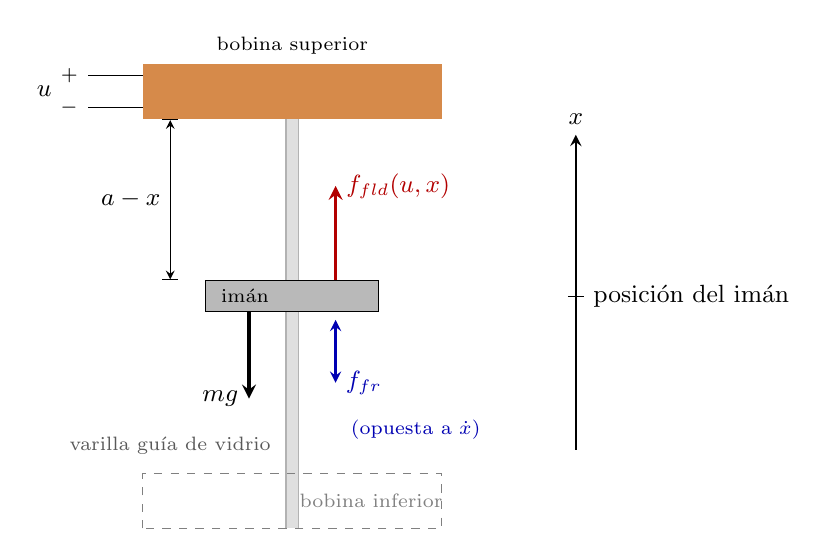
\begin{tikzpicture}[>=stealth, font=\small]
  \definecolor{cobre}{RGB}{214,138,74}
  % varilla guía
  \fill[gray!25] (-0.08,-3.6) rectangle (0.08,2.15);
  \draw[gray!60] (-0.08,-3.6) -- (-0.08,2.15) (0.08,-3.6) -- (0.08,2.15);
  \node[gray!70!black, anchor=east, font=\scriptsize] at (-0.15,-2.55) {varilla guía de vidrio};
  % bobina superior (activa)
  \fill[cobre] (-1.9,1.6) rectangle (1.9,2.3);
  \node[above, font=\scriptsize] at (0,2.3) {bobina superior};
  \draw (-1.9,2.15) -- (-2.6,2.15) node[left, font=\scriptsize] {$+$};
  \draw (-1.9,1.75) -- (-2.6,1.75) node[left, font=\scriptsize] {$-$};
  \node at (-3.15,1.95) {$u$};
  % bobina inferior (inactiva en esta configuración)
  \draw[dashed, gray] (-1.9,-3.6) rectangle (1.9,-2.9);
  \node[gray, font=\scriptsize] at (1.0,-3.25) {bobina inferior};
  % imán levitante
  \fill[gray!55] (-1.1,-0.85) rectangle (1.1,-0.45);
  \draw (-1.1,-0.85) rectangle (1.1,-0.45);
  \node[font=\scriptsize] at (-0.6,-0.65) {imán};
  % fuerzas
  \draw[->, very thick, red!70!black] (0.55,-0.45) -- (0.55,0.75) node[right] {$f_{\text{fld}}(u,x)$};
  \draw[->, very thick] (-0.55,-0.85) -- (-0.55,-1.95) node[left] {$mg$};
  \draw[<->, thick, blue!70!black] (0.55,-0.95) -- (0.55,-1.75) node[right] {$f_{\text{fr}}$};
  \node[blue!70!black, font=\scriptsize, anchor=north west] at (0.62,-2.1) {(opuesta a $\dot x$)};
  % distancia a la bobina
  \draw[|<->|, thin] (-1.55,-0.45) -- (-1.55,1.6) node[midway, left] {$a-x$};
  % eje x
  \draw[->, thick] (3.6,-2.6) -- (3.6,1.4) node[above] {$x$};
  \draw (3.5,-0.65) -- (3.7,-0.65) node[right] {posición del imán};
\end{tikzpicture}

    \caption[Esquema del ECP-730 en configuración atractiva]{Esquema del sistema de levitación ECP-730 en configuración atractiva. La bobina superior atrae al imán, que se desliza sobre una varilla guía; el contacto entre ambos produce la fricción $f_{\text{fr}}$. La bobina inferior solo se emplea en la configuración repulsiva.}
    \label{fig:dispositivo}
\end{figure}

\section{\texorpdfstring{Fuerza electromagnética $f_{\text{fld}}$}{Fuerza electromagnética}}\label{sec:fuerza}

La literatura documenta varias formas no lineales para la fuerza electromagnética, que dependen de cómo varía la inductancia de la bobina con la posición del objeto levitante. De acuerdo con Al-Muthair y Zribi~\cite{al}, la fuerza sobre una bola ferromagnética levitada se aproxima por
\begin{equation}
f_{\text{fld}} = C\left(\dfrac{i}{x}\right)^2 .
\label{eq:fld_al}
\end{equation}
En la aproximación de Al-Muthair~\eqref{eq:fld_al}, la fuerza crece con el cuadrado de la intensidad de corriente $i$ y decrece con el cuadrado de la posición $x$ de la bola. La constante $C$ de la fuerza magnética reúne las propiedades del electroimán.

Charara et al.~\cite{charara} calculan la fuerza electromagnética dentro de un cojinete magnético como
\begin{equation}
f_{\text{fld}} = K\,\frac{\operatorname{sign}(i)\,i^{2}}{e^{2}},
\qquad
K = 0{,}25 \cos\!\left(\frac{\pi}{8}\right)\!\mu\, n^{2} S .
\label{eq:fld_charara}
\end{equation}
En el modelo del cojinete~\eqref{eq:fld_charara}, la fuerza conserva el signo de la corriente $i$ y decrece con el cuadrado del entrehierro $e$. La constante $K$ depende del área $S$ de la cara del polo, de la permeabilidad magnética del vacío $\mu$ y del número $n$ de vueltas del embobinado.

El Hajjaji y Ouladsine~\cite{el} determinaron experimentalmente que la fuerza electromagnética sobre una esfera metálica tiene la forma
\begin{equation}
f_{\text{fld}} = \dfrac{i^{2}}{b_0 + b_1x + b_2x^3 + b_3x^4} .
\label{eq:fld_hajjaji}
\end{equation}
Los coeficientes del ajuste experimental~\eqref{eq:fld_hajjaji} son $b_0=0{,}0304$, $b_1=0{,}7159$, $b_2=-0{,}9165$ y $b_3=1{,}1994$.

Zhao et al.~\cite{zhao} calculan la fuerza del electroimán que hace levitar una bola metálica como
\begin{equation}
f_{\text{fld}} = \frac{L_0 x_0 i^2}{2x^2} .
\label{eq:fld_zhao}
\end{equation}
La fuerza del modelo de Zhao~\eqref{eq:fld_zhao} crece con el cuadrado de la corriente $i$ del embobinado y decrece con el cuadrado de la posición $x$ de la bola. Su escala la fija la inductancia $L_0$ del sistema en el punto de equilibrio $x_0$.

Zhang y Suyama~\cite{feifei} determinan, para un sistema similar, la fuerza electromagnética
\begin{equation}
f_{\text{fld}} = \frac{K i^2}{(H - x)^2} .
\label{eq:fld_zhang}
\end{equation}
La fuerza del modelo de Zhang~\eqref{eq:fld_zhang} también crece con el cuadrado de la intensidad de la corriente $i$, y su denominador depende de la posición $x$ del objeto. Las constantes $K$ y $H$ son parámetros del sistema.

Cada uno de estos modelos está condicionado por la configuración del sistema y por la metodología, analítica o experimental, con que se obtuvo. Por ello, en este trabajo se adopta el modelo del levitador ECP-730 que da el fabricante en su hoja de especificaciones~\cite{parks}, validado experimentalmente por Hernández Alcántara et al.~\cite{alcantara},
\begin{equation}
f_{\text{fld}} = \frac{u}{b(a-x)^4} .
\label{eq:fld}
\end{equation}
La fuerza del fabricante~\eqref{eq:fld} es proporcional al voltaje $u$ aplicado en las terminales del embobinado del electroimán y decrece con la cuarta potencia de la distancia $a-x$ entre el imán, en la posición $x$, y la bobina. Los parámetros $a$ y $b$ son propios del dispositivo y se reúnen en la tabla~\ref{tab:parametros}.

Con la fuerza del fabricante, el imán en reposo y sin fricción permanece en equilibrio en la posición $x$ cuando el voltaje es
\begin{equation}
u_e(x) = mg\,b\,(a-x)^4 .
\label{eq:ue}
\end{equation}
El voltaje de equilibrio~\eqref{eq:ue} es el que hace que la fuerza electromagnética compense el peso. Crece con la cuarta potencia de la distancia a la bobina, y la zona muerta del actuador, que se describe en la sección~\ref{sec:zm_modelo}, se centra en él.

\section{Fricción con atascamiento-deslizamiento}\label{sec:friccion_modelo}

La sección~\ref{sec:fund_friccion} describió las componentes de la fricción y el método de Karnopp en general. Esta sección precisa cómo se aplican al imán.

En este trabajo se emplea un modelo de fricción compuesto. Con velocidad nula, el imán está en régimen de fricción estática; cuando la fuerza externa lo pone en movimiento, la fricción disminuye de golpe y pasa al régimen de fricción dinámica. La fuerza de fricción es
\begin{equation}
f_{\text{fr}} =
\begin{cases}
m\,c_1\,v,
& v \neq 0, \\[6pt]
\min\!\left(|F_e|,\,F_s\right)\,\operatorname{sign}(F_e),
& v = 0 .
\end{cases}
\label{eq:friccion}
\end{equation}
En el régimen de deslizamiento, la fricción~\eqref{eq:friccion} es viscosa y proporcional a la velocidad $v$ del imán, con el coeficiente $c_1$ de fricción viscosa por unidad de masa. En reposo, la fricción equilibra la fuerza externa $F_e(t)$ que actúa sobre el imán, es decir, la suma de la fuerza electromagnética y el peso, hasta un valor máximo $F_s$, la fricción estática máxima.

La discontinuidad de la fricción en la velocidad cero es una dificultad más numérica que física, y existe una amplia variedad de estrategias para implementarla, conocidas como modelos dinámicos de fricción~\cite{haessig}. Aquí se emplea el método de Karnopp~\cite{karnopp}, por su fácil implementación. Con él, el imán se considera detenido mientras su velocidad cumple $|v| \le DV$, con la banda de velocidad nula $DV$ de la tabla~\ref{tab:parametros}, y la ecuación~\eqref{eq:friccion} decide si la fuerza externa lo mantiene atascado o lo libera.

\section{Zona muerta centrada en el voltaje de equilibrio}\label{sec:zm_modelo}

Pérez-Gómez~\cite{perez} sostiene que la zona muerta dura describe con mayor precisión el fenómeno observado en motores eléctricos, en los que esta no linealidad se centra en $u_e(t) = 0$, el único voltaje de equilibrio de los sistemas de control de posición angular.

En los sistemas de levitación magnética, en cambio, cada posición tiene su propio voltaje de equilibrio $u_e$~\eqref{eq:ue}, y la zona muerta se centra en él,
\begin{equation}
v(t) = D\big(u(t)\big) =
\begin{cases}
m_r \big(u(t) - u_e - b_r\big) - h_r, & u(t) - u_e \ge b_r, \\[6pt]
0, & b_l < u(t) - u_e < b_r, \\[6pt]
m_l \big(u(t) - u_e - b_l\big) - h_l, & u(t) - u_e \le b_l.
\end{cases}
\label{eq:zm}
\end{equation}
La zona muerta~\eqref{eq:zm} transforma el voltaje comandado $u$ en la salida $v$ del actuador. En esta ecuación, y en la figura~\ref{fig:zm} y el lazo de la figura~\ref{lazo_de_control_con_zm}, $v$ denota la salida de la zona muerta y no la velocidad del imán, que en el resto del capítulo se designa con el mismo símbolo. Mientras la desviación $u-u_e$ permanece entre los umbrales $b_l$ y $b_r$, la salida es nula. Fuera de esa banda, la salida crece con las pendientes $m_r$ y $m_l$ y se desplaza por los saltos $h_r$ y $h_l$. Estos seis parámetros son desconocidos, pero sus signos se conocen: $m_r > 0$, $m_l > 0$, $b_r > 0$, $b_l < 0$, $h_r < 0$ y $h_l > 0$.


\begin{figure}[ht]
    \centering
    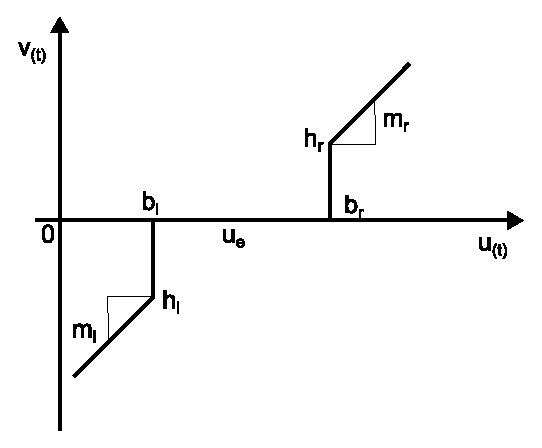
\includegraphics[width=0.45\textwidth]{images/chapter_1/zm_levitador.eps}
    \caption[Zona muerta centrada en el voltaje de equilibrio]{Zona muerta $v=D(u)$ centrada en el voltaje de equilibrio $u_e$, con pendientes $m_l$, $m_r$, umbrales $b_l$, $b_r$ y saltos $h_l$, $h_r$.}
    \label{fig:zm}
\end{figure}

La figura~\ref{fig:zm} muestra la forma de $D(u)$: mientras el voltaje comandado se mantenga dentro de la banda $(u_e+b_l,\,u_e+b_r)$, la salida $v$ del actuador es nula.

Como los parámetros de $D(u)$ no se conocen para el ECP-730, en las simulaciones se emplea una implementación simplificada con la misma asimetría de signos. Mientras el imán está en movimiento, el actuador no responde a cambios del voltaje comandado comprendidos entre $-0{,}02$ y $+0{,}025$~V respecto al último voltaje aplicado, que se mantiene; los cambios mayores se transmiten sin modificación. Cuando el imán está atascado, el voltaje comandado se aplica directamente. Esta implementación no es equivalente a $D(u)$. Tiene memoria, porque compara con el último voltaje aplicado en lugar de con $u_e$, y se desactiva mientras el imán está atascado. Los resultados de simulación valen, por tanto, para esta retención de voltaje y no para una zona muerta estática identificada del ECP-730. En una simulación adicional sin zona muerta, el ciclo límite del PII persiste con una amplitud un 8\,\% menor, de modo que la oscilación no necesita esta retención para aparecer. La identificación de los parámetros de $D(u)$ se propone como trabajo futuro.

La figura~\ref{lazo_de_control_con_zm} muestra el lazo de control completo, con la zona muerta entre el controlador y la planta.

\begin{figure}[ht]
    \centering
       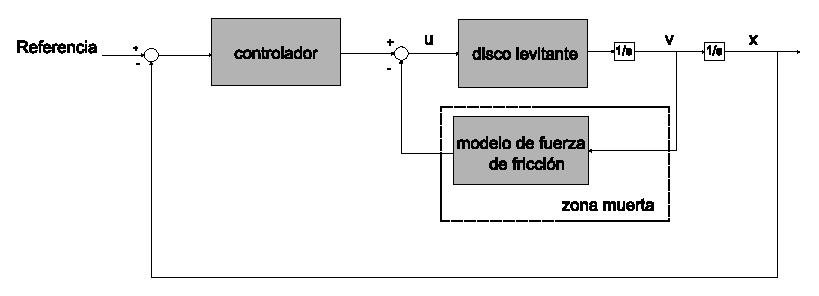
\includegraphics[width=0.6\textwidth]{images/chapter_1/lazo_de_control_con_zm.eps}
    \caption{Lazo de control con zona muerta}
    \label{lazo_de_control_con_zm}
\end{figure}

\section{Parámetros del modelo}\label{sec:parametros}

Los parámetros del modelo no lineal ($a$, $b$, $c_1$, $m$, $g$) fueron identificados experimentalmente por Hernández Alcántara~\cite{diana_tesis} para el dispositivo ECP-730 en configuración repulsiva (estable en lazo abierto), mediante ensayos de estado estacionario y respuesta dinámica en lazo abierto. En el presente trabajo se adoptan esos mismos parámetros y se aplican a la configuración atractiva (inestable en lazo abierto), en la que la bobina superior atrae al imán. La estructura funcional del modelo es idéntica en ambas configuraciones; en la atractiva, la fuerza magnética crece al disminuir la brecha entre el imán y la bobina, lo que hace que los puntos de equilibrio sean inestables.

La tabla~\ref{tab:parametros} reúne estos valores junto con los parámetros del modelo de fricción, el intervalo de la señal de control y la banda de la zona muerta simulada. Las fuerzas se expresan en $\text{kg}\cdot\text{cm}/\text{s}^2$, unidades en las que el peso del imán es $mg = 138{,}3$. En la tesis de Hernández Alcántara~\cite{diana_tesis}, $c_1$ se reporta en $\text{kg}^{-1}$; dado que multiplica a la velocidad en la ecuación de aceleración, sus unidades consistentes son $\text{s}^{-1}$. Por la misma razón, el valor de $b$ corresponde a fuerzas en $\text{kg}\cdot\text{cm}/\text{s}^2$, es decir, a voltios por $(\text{kg}\cdot\text{cm}/\text{s}^2)\cdot\text{cm}^4$. Ese antecedente lo reporta en $\text{V}/(\text{N}\cdot\text{cm}^4)$, y con esa unidad el valor equivalente sería $1{,}6163\times10^{-4}$, cien veces mayor. Con el valor y la unidad de la tabla~\ref{tab:parametros}, el modelo reproduce los voltajes de equilibrio que se usan en todo el trabajo.


\begin{table}[ht]
\centering
\caption{Parámetros del modelo}
\label{tab:parametros}
\begin{tabular}{|c|c|l|}
\hline
$a$ & $7{,}17184\;[\text{cm}]$ & parámetro de la fuerza electromagnética \\ \hline
$b$ & $1{,}6163 \times 10^{-6}\;[\text{V}\cdot\text{s}^2/(\text{kg}\cdot\text{cm}^5)]$ & parámetro de la fuerza electromagnética \\ \hline
$c_1$ & $8{,}563\;[\text{s}^{-1}]$ & fricción viscosa por unidad de masa \\ \hline
$m$ & $0{,}141\;[\text{kg}]$ & masa del imán \\ \hline
$g$ & $981\;[\text{cm}/\text{s}^2]$ & aceleración de la gravedad \\ \hline
$F_s$ & $20\;[\text{kg}\cdot\text{cm}/\text{s}^2]$ ($0{,}2$~N) & fricción estática máxima (Karnopp) \\ \hline
$DV$ & $0{,}02\;[\text{cm}/\text{s}]$ & banda de velocidad nula (Karnopp) \\ \hline
$u$ & $[0;\ 3{,}5]\;[\text{V}]$ & intervalo de la señal de control \\ \hline
$[b_l,\,b_r]$ & $[-0{,}02;\ +0{,}025]\;[\text{V}]$ & banda de la zona muerta simulada \\ \hline
\end{tabular}
\end{table}

\section{Modelo linealizado}\label{sec:linealizado}

Para diseñar el controlador se linealiza el modelo alrededor de una posición de equilibrio $x_1^{\ast}$, con el procedimiento general de la sección~\ref{sec:fund_linealizacion}. El modelo linealizado en espacio de estados para la configuración inestable es

\begin{equation}
\begin{aligned}
\dot{x}
&=
\begin{bmatrix}
0 & 1 \\[6pt]
\dfrac{4g}{(a-x_1^{\ast})} & -c_1
\end{bmatrix}x
+
\begin{bmatrix}
0 \\[6pt]
\dfrac{1}{mb\,(a-x_1^{\ast})^4}
\end{bmatrix}u,
\\[10pt]
y &= \begin{bmatrix} 1 & 0 \end{bmatrix} x .
\end{aligned}
\label{eq:lineal}
\end{equation}
En el modelo linealizado~\eqref{eq:lineal}, el vector de estado $x$ reúne la posición $x_1$ y la velocidad $x_2$ del imán, y la salida $y$ es la posición. El coeficiente $c_1$ de fricción viscosa por unidad de masa aparece en la matriz de estado como un amortiguamiento.

Su ecuación característica es
\begin{equation}
\lambda^2 + c_1\lambda - \dfrac{4g}{(a-x_1^{\ast})} = 0 .
\label{eq:caracteristica}
\end{equation}
Como $a - x_1^{\ast} > 0$ para toda posición alcanzable, el término independiente de la ecuación característica~\eqref{eq:caracteristica} es negativo y la ecuación tiene siempre una raíz real positiva: todos los puntos de equilibrio de la configuración atractiva son inestables. En $x_1^{\ast}=-4$~cm las raíces son $\lambda_1 = -23{,}5057$ y $\lambda_2 = 14{,}9427$.

Las matrices de controlabilidad y de observabilidad del modelo linealizado son
\begin{equation}
\mathcal{C}
=
\begin{bmatrix}
0 & \beta\\[6pt]
\beta & -c_1 \beta
\end{bmatrix} ,
\qquad
\mathcal{O}
=
\begin{bmatrix}
1 & 0\\[6pt]
0 & 1
\end{bmatrix} .
\label{eq:ctrb_obsv}
\end{equation}
La constante $\beta = 1/[m\,b\,(a-x_1^{\ast})^4]$ es la ganancia con la que el voltaje entra en la aceleración del imán. Las dos matrices~\eqref{eq:ctrb_obsv} tienen rango completo, de modo que el sistema es controlable y observable: con la entrada de la planta se puede llevar el estado a cualquier punto del espacio de estados, y a partir de la salida se puede determinar en qué punto se encuentra.

% Generado a partir de calculus/Final_Bien/evidencia_P8.m (simulador corregido).
\section{Comportamiento en lazo abierto}\label{sec:lazo_abierto}

Para caracterizar la inestabilidad de la configuración atractiva, se simuló el modelo no lineal sin fricción estática ni zona muerta, aplicando el voltaje de equilibrio $u=u_e(x_1^*)$ y desplazando la posición inicial $0{,}01$~cm respecto al equilibrio, en $x_1^*=-4$, $-3$ y $-2$~cm. La figura~\ref{fig:p8_lazo_abierto} muestra que la desviación crece exponencialmente y alcanza 1~cm en $0{,}33$, $0{,}32$ y $0{,}30$~s, respectivamente; el modelo linealizado reproduce el crecimiento con un tiempo de duplicación $\ln 2/\lambda_2$ de $46$, $44$ y $41$~ms. Cuanto más cerca de la bobina se encuentra el equilibrio, más rápido es el polo inestable.

\begin{figure}[ht]
    \centering
    % Estilo común de las figuras de evidencia P8 (pgfplots).
\pgfplotsset{
  pocho/.style={
    width=0.92\textwidth, height=5.2cm,
    grid=major, grid style={gray!25},
    tick label style={font=\small}, label style={font=\small}, legend style={font=\small},
    /pgf/number format/use comma,
    scaled ticks=false,
    y tick label style={/pgf/number format/fixed},
    table/col sep=comma, unbounded coords=jump,
    every axis plot/.append style={line join=round},
  },
}
\definecolor{tray}{RGB}{31,94,166}
\definecolor{refc}{RGB}{40,40,40}
\definecolor{ctl2}{RGB}{196,96,40}
\definecolor{ver}{RGB}{46,133,64}

\begin{tikzpicture}
\begin{semilogyaxis}[pocho, height=6cm, xmin=0, xmax=0.36, ymin=0.01, ymax=1,
    xlabel={tiempo [\si{s}]}, ylabel={$|x_1(t)-x_1^*|$ [\si{cm}]},
    x tick label style={/pgf/number format/fixed},
    legend style={at={(0.02,0.98)}, anchor=north west}, legend cell align=left]
  \addplot[tray, line width=1pt]  table[x=t, y=nl_m4] {images/p8_results/tikz/lazo_abierto.csv}; \addlegendentry{$x_1^*=-4$ cm}
  \addplot[ctl2, line width=1pt]  table[x=t, y=nl_m3] {images/p8_results/tikz/lazo_abierto.csv}; \addlegendentry{$x_1^*=-3$ cm}
  \addplot[ver, line width=1pt]   table[x=t, y=nl_m2] {images/p8_results/tikz/lazo_abierto.csv}; \addlegendentry{$x_1^*=-2$ cm}
  \addplot[tray, densely dashed]  table[x=t, y=lin_m4] {images/p8_results/tikz/lazo_abierto.csv}; \addlegendentry{modelo lineal}
  \addplot[ctl2, densely dashed, forget plot] table[x=t, y=lin_m3] {images/p8_results/tikz/lazo_abierto.csv};
  \addplot[ver, densely dashed, forget plot]  table[x=t, y=lin_m2] {images/p8_results/tikz/lazo_abierto.csv};
\end{semilogyaxis}
\end{tikzpicture}

    \caption[Lazo abierto en los puntos de equilibrio]{Desviación respecto al equilibrio en lazo abierto, con $u=u_e$ y una perturbación inicial de $0{,}01$~cm. Líneas continuas: modelo no lineal; discontinuas: modelo linealizado.}
    \label{fig:p8_lazo_abierto}
\end{figure}

El retrato de fase alrededor de $x_1^*=-4$~cm (figura~\ref{fig:p8_retrato}) confirma que el equilibrio es un punto silla: las trayectorias se alejan a lo largo de la variedad inestable, salvo las que parten exactamente sobre la variedad estable.


\begin{figure}[ht]
    \centering
    % Estilo común de las figuras de evidencia P8 (pgfplots).
\pgfplotsset{
  pocho/.style={
    width=0.92\textwidth, height=5.2cm,
    grid=major, grid style={gray!25},
    tick label style={font=\small}, label style={font=\small}, legend style={font=\small},
    /pgf/number format/use comma,
    scaled ticks=false,
    y tick label style={/pgf/number format/fixed},
    table/col sep=comma, unbounded coords=jump,
    every axis plot/.append style={line join=round},
  },
}
\definecolor{tray}{RGB}{31,94,166}
\definecolor{refc}{RGB}{40,40,40}
\definecolor{ctl2}{RGB}{196,96,40}
\definecolor{ver}{RGB}{46,133,64}

\begin{tikzpicture}
\begin{axis}[pocho, width=0.8\textwidth, height=7.5cm, xmin=-4.5, xmax=-3.5, ymin=-10, ymax=10,
    xlabel={posición $x_1$ [\si{cm}]}, ylabel={velocidad $x_2$ [\si{cm/s}]},
    legend style={at={(0.98,0.02)}, anchor=south east, fill=white}, legend cell align=left]
  \addplot[gray!60, quiver={u=\thisrow{dx}, v=\thisrow{dv}, every arrow/.append style={-stealth}}, forget plot]
    table[x=x, y=v] {images/p8_results/tikz/campo.csv};
  \addplot[tray, line width=0.9pt] table[x=x, y=v] {images/p8_results/tikz/trayectorias.csv}; \addlegendentry{trayectorias}
  \addplot[ctl2, line width=1.4pt] table[x=x, y=v] {images/p8_results/tikz/variedad_inestable.csv}; \addlegendentry{variedad inestable}
  \addplot[ver, line width=3pt, opacity=0.6] coordinates {(-4.4448,0) (-3.6291,0)}; \addlegendentry{banda de atascamiento ($u=u_e$)}
  \addplot[only marks, mark=*, mark size=2pt, refc] coordinates {(-4,0)}; \addlegendentry{equilibrio $x_1^*=-4$ cm}
\end{axis}
\end{tikzpicture}

    \caption[Retrato de fase en lazo abierto]{Retrato de fase del modelo no lineal sin fricción estática alrededor de $x_1^*=-4$~cm, con $u=u_e$. La banda verde indica las posiciones en las que, con el imán en reposo, la fricción estática lo mantiene atascado.}
    \label{fig:p8_retrato}
\end{figure}

Al incorporar la fricción estática de Karnopp cambia la situación en reposo: si el imán está detenido y $u=u_e$, la fuerza neta $u/[b(a-x)^4]-mg$ no supera $F_s$ mientras la posición se encuentre entre $-4{,}44$ y $-3{,}63$~cm, de modo que el imán permanece atascado en cualquier punto de esa banda. Para $x_1^*=-3$ y $-2$~cm las bandas correspondientes son $[-3{,}41;\,-2{,}66]$ y $[-2{,}37;\,-1{,}70]$~cm. La fricción estática enmascara así la inestabilidad del equilibrio mientras el imán no se mueva.

\FloatBarrier

\section{Análisis estático del actuador}\label{sec:actuador_estatico}

El voltaje que puede aplicar el actuador está acotado a $u\in[0;\,3{,}5]$~V, y esa cota determina en qué posiciones puede operar el sistema. Para sostener el imán en $x_1$ se necesita el voltaje de equilibrio~\eqref{eq:ue}, que crece rápidamente al alejarse de la bobina: $1{,}58$~V en $-2$~cm, $2{,}39$~V en $-3$~cm, $3{,}48$~V en $-4$~cm y $4{,}91$~V en $-5$~cm. Para mover el imán hay que vencer además la fricción estática, lo que exige llegar a $u_e(1\pm F_s/mg)$, es decir, a un $14{,}5$\,\% por encima o por debajo del equilibrio. La sección~\ref{sec:analisis_ciclo} retoma esta banda para explicar el ciclo límite.

En $x_1=-4$~cm, el punto en que se linealizó el modelo para el diseño, el imán puede sostenerse con $3{,}48$~V, pero no subir: para despegarlo hacia la bobina se requieren unos $3{,}99$~V, por encima de la cota de $3{,}5$~V. Sí puede despegarse hacia abajo si el voltaje baja de unos $2{,}98$~V, pero entonces se aleja de la bobina, el voltaje de equilibrio crece todavía más y el actuador ya no puede recuperarlo. Desde $-4$~cm el imán no tiene, por tanto, ningún movimiento regulable, aunque sí puede caer. El barrido de escalones del capítulo~\ref{chap:desempeno} determina qué posiciones y qué cambios de referencia son alcanzables con $u\le3{,}5$~V, y de él se obtiene el intervalo de pruebas.

El modelo queda así completo: una planta inestable en lazo abierto, con fricción estática que puede mantener al imán detenido y un actuador acotado, con zona muerta, que limita dónde se puede actuar. Sobre el modelo linealizado se diseña, en el capítulo siguiente, el controlador.
